\documentclass[sigconf, nonacm]{acmart}

\newcommand{\scream}[2]{{\color{red} \textbf{#1}: #2}}
\newcommand{\mihai}[1]{\scream{MIHAI}{#1}}
\newcommand{\multilinecomment}[1]{}
\usepackage{listings}
\usepackage{hyperref}
\usepackage{url}
\usepackage{listofitems}
% control over list layout
\usepackage{enumitem}
\setlist{noitemsep,leftmargin=*}


\lstdefinelanguage{ddlog}{
  language=Java, % we base it on Java, just for comments
  morekeywords={input, output, relation, typedef, bool, not,
    string, bit, extern, function, var, for, match, in, integer, % not really in DDlog
    Aggregate, FlatMap},
  deletestring=[b]{'}
}
\lstdefinelanguage{p4}{
  language=Java, % we base it on Java, just for comments
  morekeywords={table, typedef, bool, string, bit,
  extern, function, match, in, int, out, inout, true, false,
  exact, optional, actions}
}
\hypersetup{
  colorlinks   = true,    % Colours links instead of ugly boxes
  urlcolor     = blue,    % Colour for external hyperlinks
  linkcolor    = blue,    % Colour of internal links
  citecolor    = red      % Colour of citations
}
\hypersetup{final}

\acmJournal{TOG}
\acmVolume{37}
\acmNumber{4}
\acmArticle{111}
\acmMonth{8}

%\citestyle{acmauthoryear}

\title[Nerpa]{Nerpa: Network Programming with Relational and Procedural Abstractions}

\author{Debnil Sur, Ben Pfaff, Leonid Ryzhyk, and Mihai Budiu}
\email{{dsur, bpfaff, lryzhyk, mbudiu}@vmware.com}
\affiliation{\institution{VMware} \country{} \city{}}

\renewcommand{\shortauthors}{Sur, et al.}

\begin{document}

\begin{abstract}
We introduce Nerpa, a new methodology for building programmable networks. Nerpa automates many aspects of the process of programming the network stack. To aid correctness, it ensures type safety across the management, control, and data planes. To improve scalability, an incremental control plane recomputes state in response to network configuration changes. We have published an implementation and examples.
\end{abstract}

\maketitle

\section{Introduction}
In the most popular approach for programming networks, the developer separately programs the management, control, and data planes. In a common approach, the management plane is implemented as an API backed by a database, the control plane as an SDN controller written in an imperative language such as Java or C++, and the data plane using flow-programmable switch software or hardware~\cite{casado-sigcomm07, gude-ccr08, koponen-osdi10, berde-hotsdn14, koponen-nsdi14, ovn-austin, NSX}.

We have identified two primary challenges in our experience building systems in this form.
\textbf{Correctness} is the first challenge. The control plane typically programs the network by issuing installing small program fragments, e.g.~OpenFlow flows, in network devices. The controller serves as a specialized compiler converting policies into these program fragments. As an SDN system adds features over time, flow rule fragments for various tables and priorities end up scattered across a large codebase. It becomes difficult for the developer to be confident of overall correctness across the feature combination matrix.

\textbf{Scalability} is the second challenge: as the system grows, the SDN controller must still respond quickly to changes. In return, this demands \textbf{incrementality}. In response to a change, the controller should not recompute and redistribute the entire network state. Instead, the recomputation should be proportional to the amount of modified state. Writing an incremental controller in an imperative language such as Java or C++ demands either an unnatural coding style or ad hoc, fragile support for incremental changes that seem important in practice~\cite{ovn-incremental, moats16}.

We present Nerpa, a prototype of a programming framework intended to address these classes of issues. To address correctness, Nerpa pairs the DDlog control plane with a P4 data plane to write a complete type-checked program. This provides more obvious correctness than an OpenFlow-like data plane. While the latter has some structure, it is not apparent to the controller, which just generates program fragments. To address scalability, the programmer writes a Nerpa control plane in Differential Datalog, or DDlog for short, a declarative language whose implementation is fully and automatically incremental~\cite{ryzhyk-datalog19}. Our implementation is available as an open-source project with an MIT license at \url{https://github.com/vmware/nerpa}, including a tutorial and a demo application.

\begin{figure}
    \centering
    \makebox[\columnwidth][c]{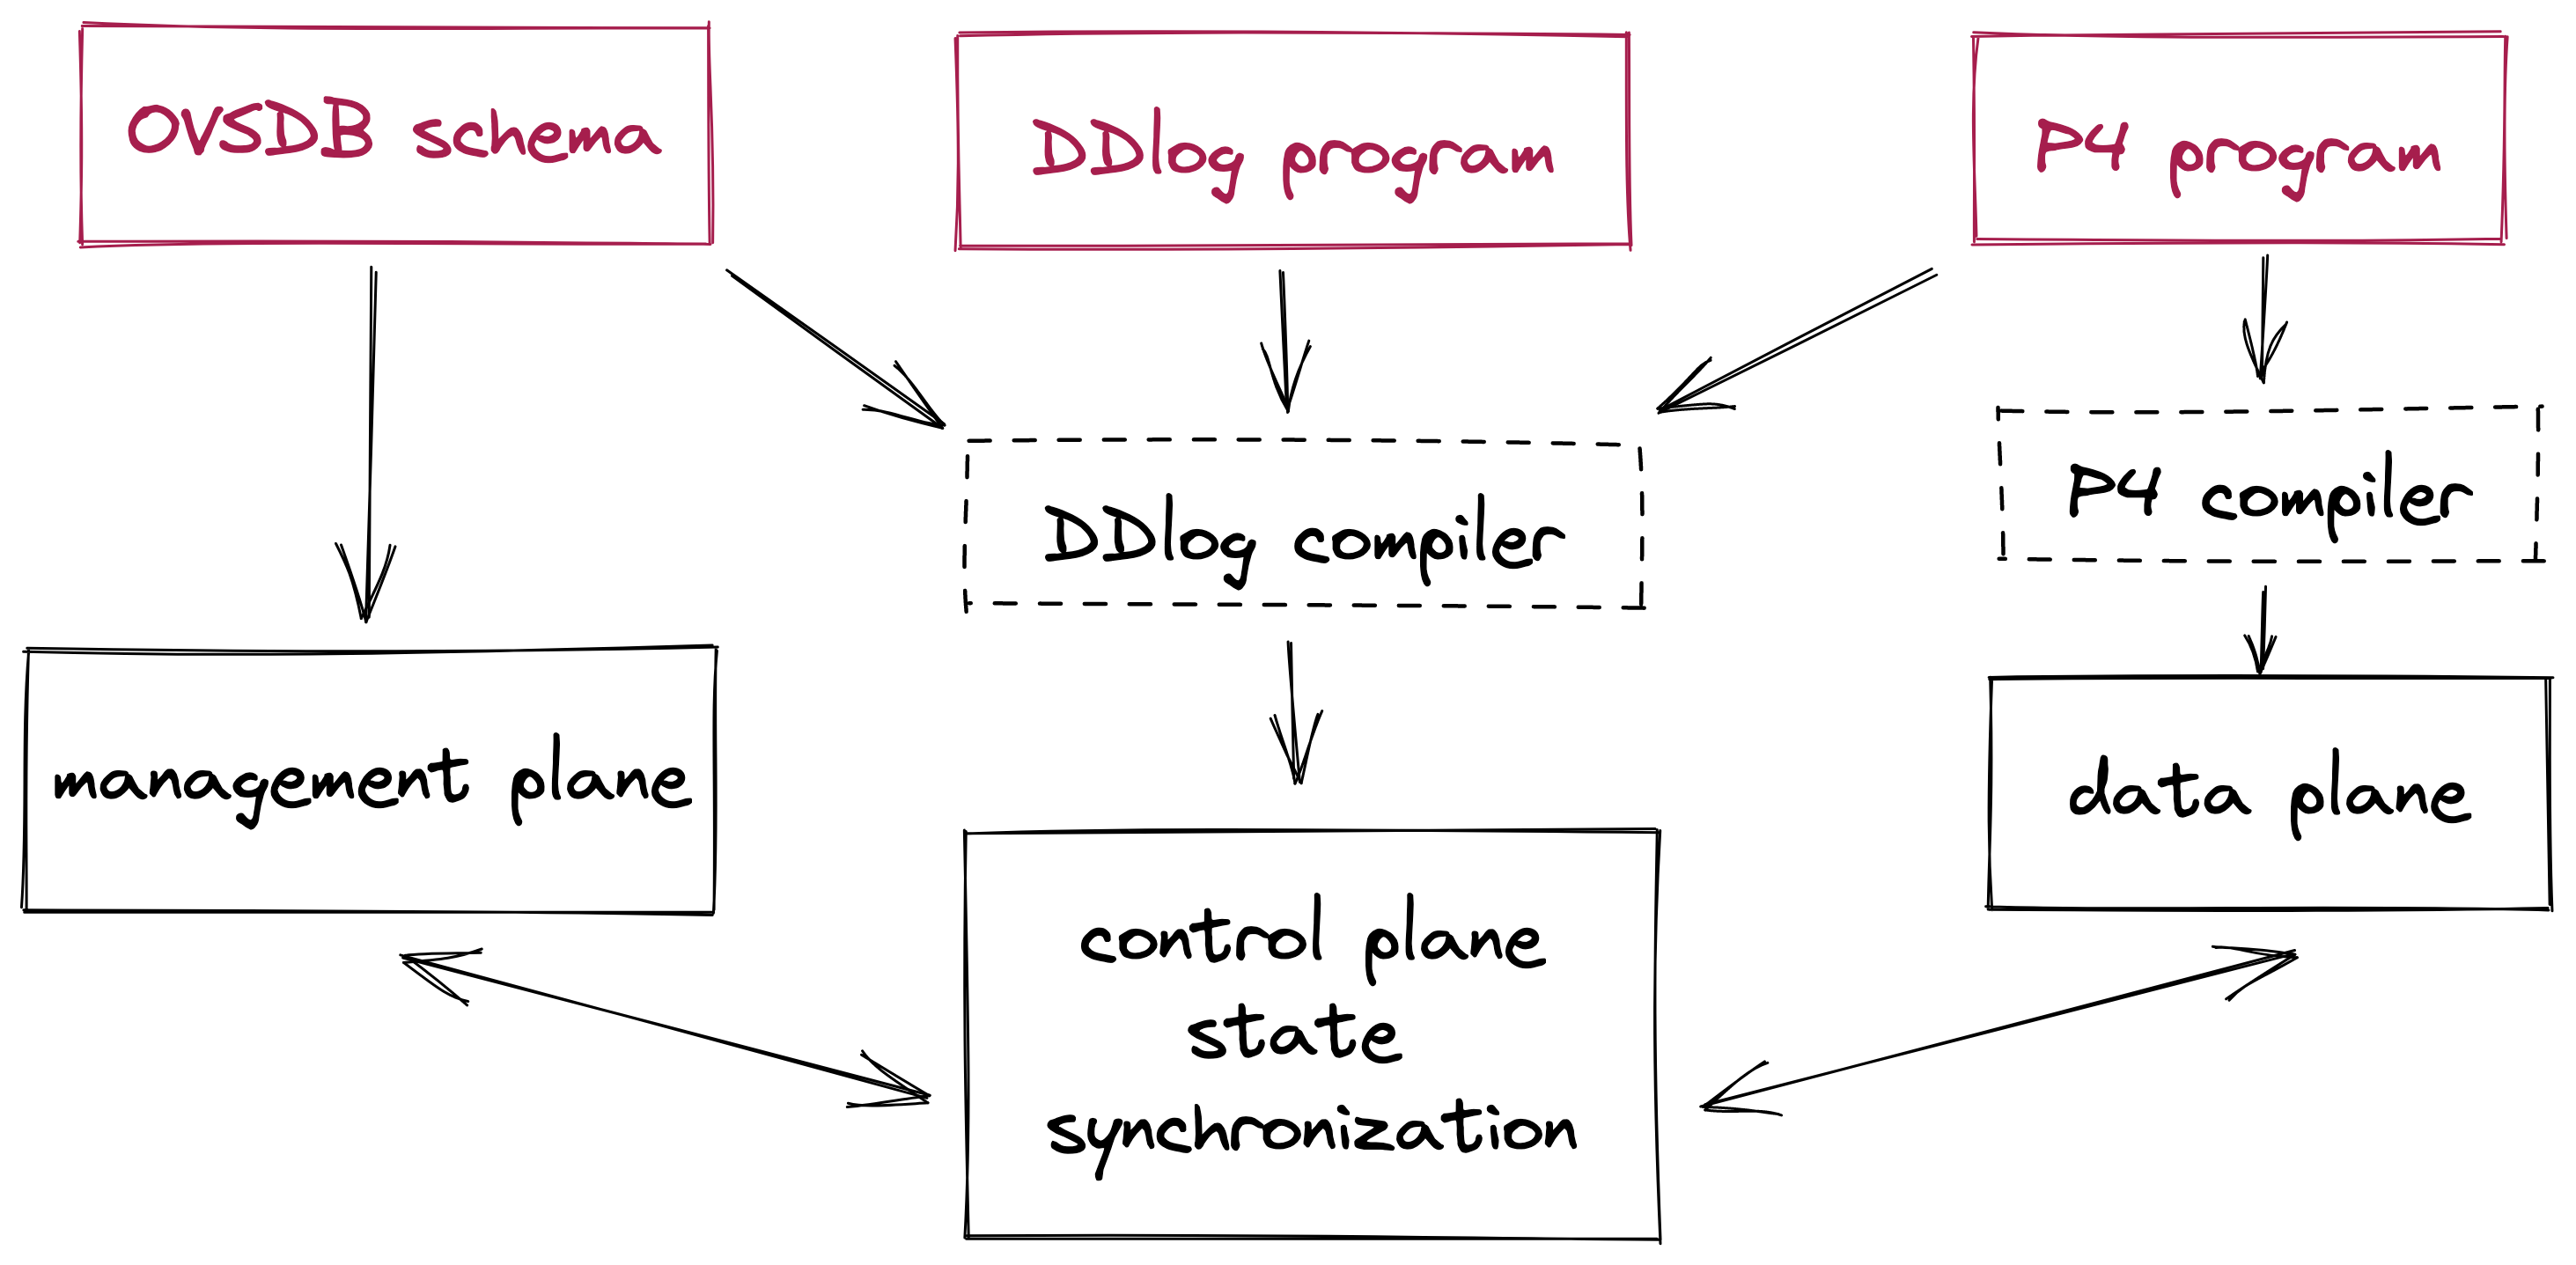
\includegraphics[width=\columnwidth]{nerpa_vision_colored.png}}
    \caption{The vision for Nerpa. The network programmer writes the red boxes. }
    \label{fig:nerpa-vision}
\end{figure}

\section{Design}

The Nerpa programming framework coordinates three pieces of software. These
correspond to the three classes of computations executed by
network devices:
\begin{description}
    \item[Management plane:] The system administrator configures the
    Nerpa management plane by populating and modifying
    the contents of an Open vSwitch Database (OVSDB) instance. Its schema represents the high-level structure of the
    network.
    \item[Control plane:] A DDlog program computes a set of output relations from the contents of some input relations. The Nerpa DDlog program has two kinds of
    input relations: (1) representing
    the current network configuration, synchronized from the management database and
    (2) representing notifications from data plane
    packets and events.  The control plane output relations correspond to
    entries for P4 tables.  The Nerpa programmer implements the control plane program
    to compute the output
    relations as a function of the input relations.  The DDlog compiler automatically
    makes this computation an incremental process.
    \item[Data plane:] The data plane is programmed using P4. The Nerpa controller
    uses the P4Runtime API to install DDlog output relations as table entries in the P4-enabled switch.
\end{description}

A Nerpa programmer supplies three files, as shown in Figure~\ref{fig:nerpa-vision}: an OVSDB schema, which defines the management plane; a DDlog program, whose rules define the control plane; and a P4 program, which implements the data plane. To interface between these software programs, Nerpa automates many tasks that previously required writing glue code, by generating the code that orchestrates the data movement between the planes. To facilitate this, DDlog input and output relations are generated from the OVSDB schema and the compiled P4 program. The Nerpa controller reads changes from OVSDB and transforms them to inputs to the DDlog program. It also transforms DDlog outputs into P4 table entries, and writes those entries to the switch using the P4Runtime API.  When the P4 program sends a digest back to the Nerpa controller, the controller
transforms it into input to a DDlog relation whose contents can also influence the controller's behavior, forming a feedback loop.  In the
compilation process, Nerpa typechecks the data definitions and ensures that only well-formed messages are exchanged.


\section{Implementation}
We describe some details of our current prototype implementation.

\subsection{Language-Specific Tooling}
The glue layers between all these services are all written in Rust. Rust's low-level control and memory safety fit Nerpa's goals well. DDlog
programs are also compiled to Rust by the DDlog compiler; DDlog is in the core of the Nerpa stack. As a result, we built Rust libraries for interfacing with OVSDB and P4Runtime.
The OVSDB Rust library uses the Rust \texttt{bindgen} crate to generate Rust foreign-function interface bindings to OVSDB’s C codebase.
The P4Runtime Rust library uses the P4Runtime Protocol Buffer definition files to generate Rust code for the API calls. It then exposes an end user friendly API. Both libraries are included in the Nerpa repository. We hope other projects in the P4 ecosystem find them useful.

\subsection{Control and Data Plane Co-Design}

Data exchange between the different planes requires an intermediate data representation.
The control plane reads input changes from the management plane and writes output changes to the data plane. The data plane can also send notifications to the control plane, as in MAC learning. In Nerpa, changes from the management plane are represented by changes in OVSDB state. Communication between the control plane and data plane uses the P4Runtime API. A packet digest can be used to send notifications to the control plane over the Stream RPC. Output changes modify entries in the match-action tables using the Write RPC.

Since all communication flows through the control plane, DDlog relations serve as the natural intermediate data representation. To represent inputs from the management plane we used \texttt{ovsdb2ddlog}, a tool which generates DDlog relations from an OVSDB schema. We
implemented \texttt{p4info2ddlog}, a tool to generate DDlog relations from a P4 program. It consumes the ``P4info'' binary file,
produced by the p4 compiler, describing the tables and other objects in the P4 program. From this, \texttt{p4info2ddlog}
generates an input relation for each packet digest and an output relation for each match-action table.
It also generates helper functions in Rust to convert data between P4Runtime and DDlog types.
This approach enables co-design of the control plane and data plane and a close integration between the two.

\subsection{Example: Simple Network Virtual Switch}

\begin{figure}
    \centering
    \makebox[\columnwidth][c]{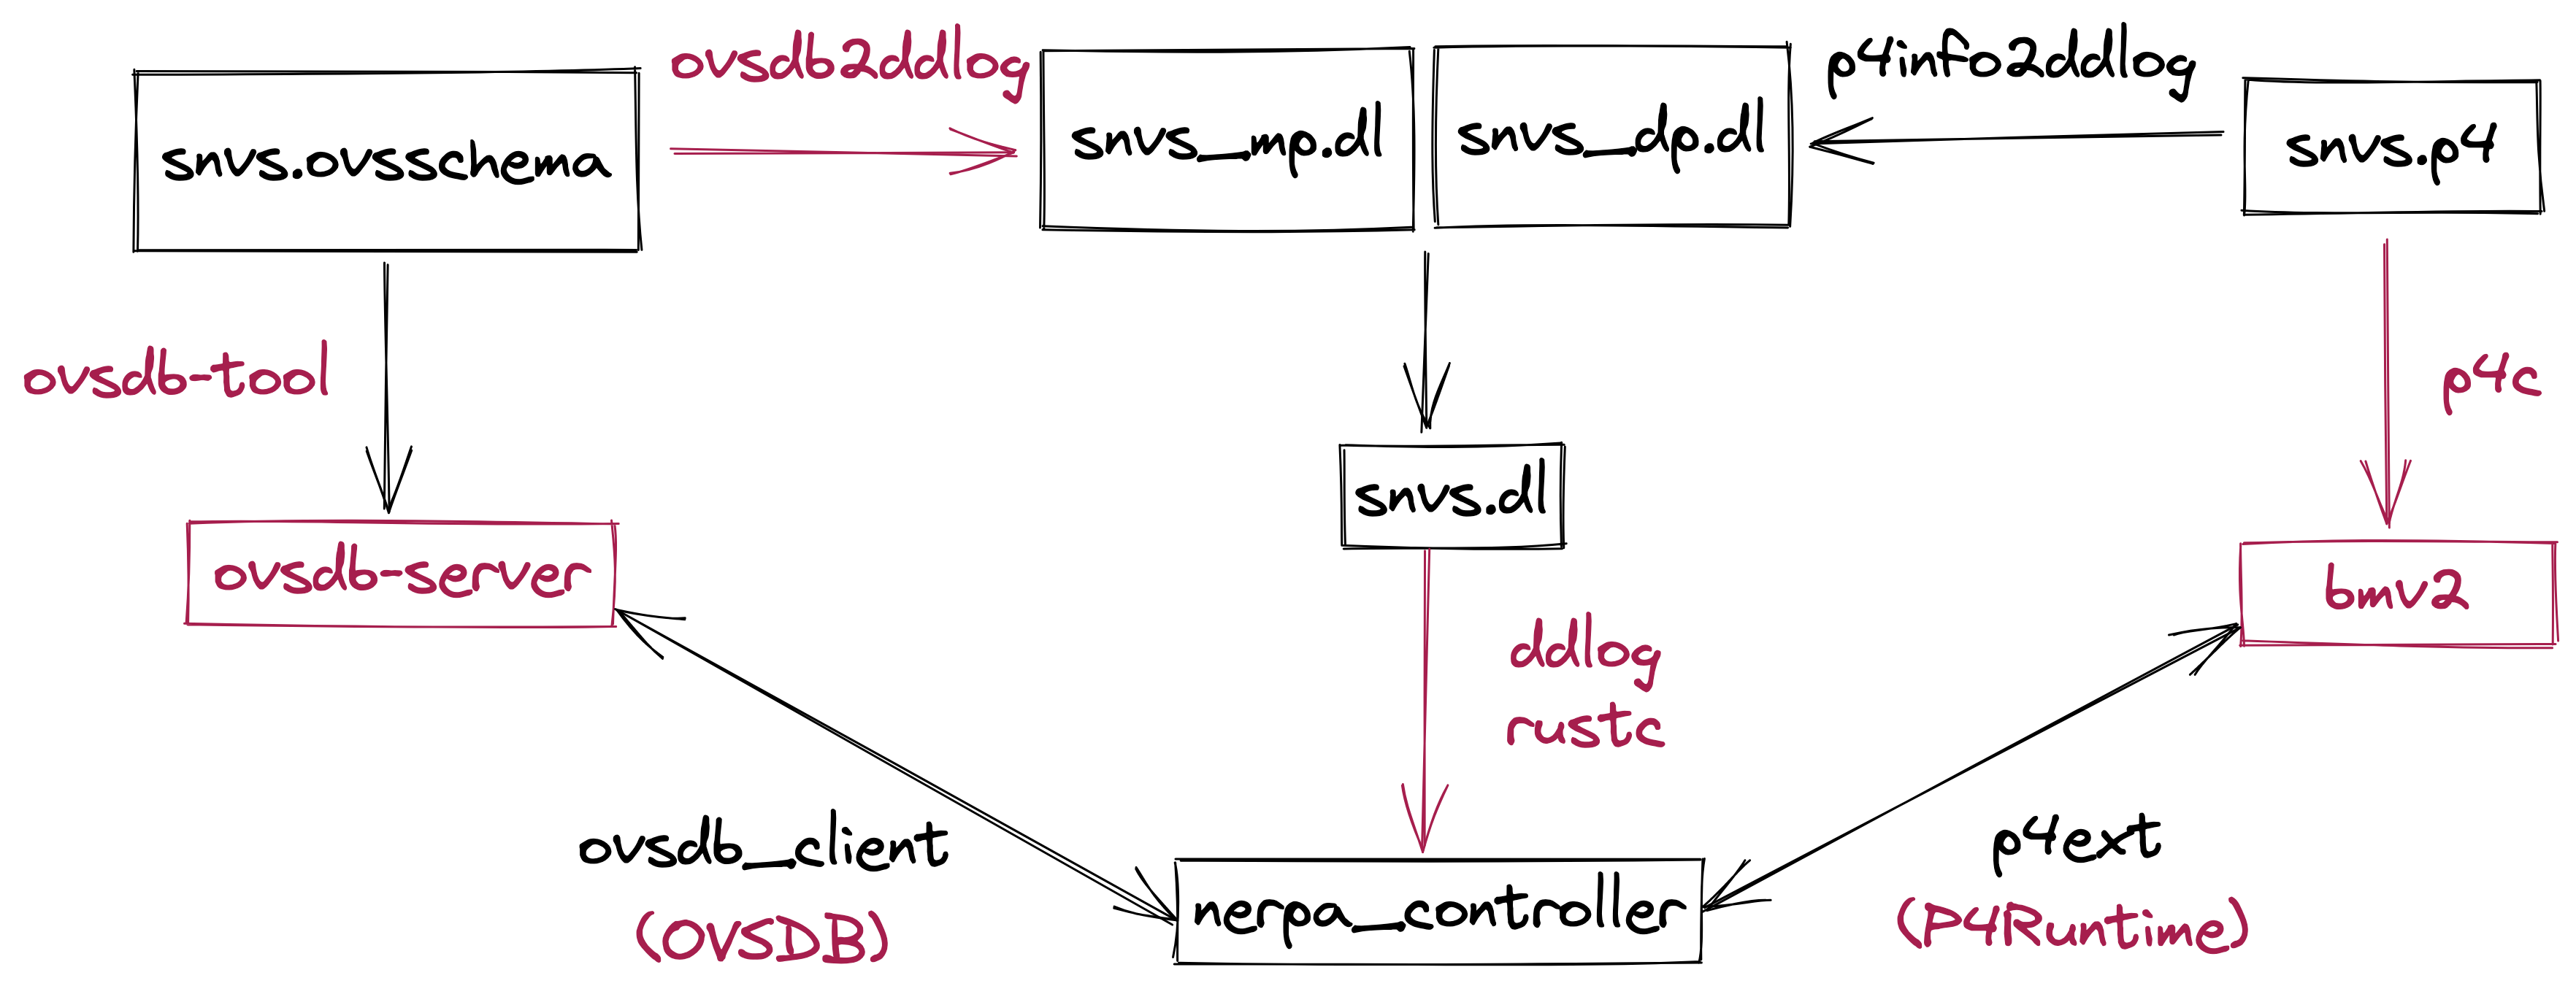
\includegraphics[width=\columnwidth]{snvs_diagram.png}}
    \caption{The \texttt{snvs} example program as processed by Nerpa. Black text represents a tool or program written as part of Nerpa, while red represents an external program.}
    \label{fig:snvs-diagram}
\end{figure}

The Nerpa repository includes a simple network virtual switch as an example implemented in Nerpa, called \texttt{snvs}.
This implements several important networking features, including VLANs, MAC learning, and port mirroring.
The Nerpa integration test executes all layers of the stack, using OVSDB, the DDlog runtime, and the P4 behavioral
simulator BMv2.

The code snippets below implement a very simplified version of the VLAN assignment feature. We generate an output relation from a P4 match-action table and an input relation from an OVSDB table. A Datalog rule then derives the output relation from the input relation. This shows how Nerpa's pieces fit together.

\lstset{
basicstyle=\tiny,
frame=single,
tabsize=2,
breaklines=true
}
\noindent\begin{minipage}{.48\columnwidth}
\begin{lstlisting}[title=P4 match-action table,frame=tlrb,language=p4]
table InVlan {
  key = {
    std_meta.in_port: exact @name("port");
    hdr.vlan.isValid(): exact @name("has_vlan") @nerpa_bool;
    hdr.vlan.vid: optional @name("vid");
  }
  actions = {
    Drop;
    SetVlan;
    UseTaggedVlan;
  }
}
\end{lstlisting}
\end{minipage}\hfill
\begin{minipage}{.48\columnwidth}
\begin{lstlisting}[title=DDlog output relation generated from the P4 program,frame=tlrb,language=ddlog]
typedef InVlanAction =
  InVlanActionDrop
| InVlanActionSetVlan{vid: bit<12>}
| InVlanActionUseTaggedVlan

output relation InVlan(
  port: bit<9>,
  has_vlan: bool,
  vid: Option<bit<12>>,
  priority: bit<32>,
  action: InVlanAction
)
\end{lstlisting}
\end{minipage}

\noindent\begin{minipage}{.48\columnwidth}
\begin{lstlisting}[title=OVSDB schema,frame=tlrb]
"Port": {
  "columns": {
    "id": {"type": {"key": {"type": "integer"}}},
    "tag": {"type": {"key": {"type": "integer"}, "min": 0, "max": 1}},
  },
}
\end{lstlisting}
\end{minipage}\hfill
\begin{minipage}{.48\columnwidth}
\begin{lstlisting}[title=DDlog input relation generated from the OVSDB schema,frame=tlrb,language=ddlog]
input relation Port (
    _uuid: uuid,
    id: integer,
    tag: Option<integer>,
)
primary key (x) x._uuid
\end{lstlisting}
\end{minipage}

\begin{lstlisting}[title=DDlog rule for VLAN assignment written by programmer,frame=tlrb,language=ddlog]
InputVlan(port,false,None,1,InputVlanActionSetVlan{vid}) :-
  Port(.id = port, .tag = tag),
  var vid = match tag {
    None -> 0,
    Some{tag} -> tag
  }.
\end{lstlisting}

\section{Conclusions}
Nerpa uses relational and procedural abstractions to improve the correctness and scalability of network programs. OVSDB and the DDlog data representation are used in the relational, incrementally programmed control plane. This is co-designed with the imperative data plane program, written in P4. We have provided a prototype and example program of a simple network virtual switch. In future, we plan to implement increasingly complex network programs.

\bibliographystyle{plain}
\bibliography{ovn}

\end{document}
